In this section we will use our gnuradio flow to perform a \gls{mitm} attack on our two feathers, as shown in \cref{mitm}.

\centrefigurestart
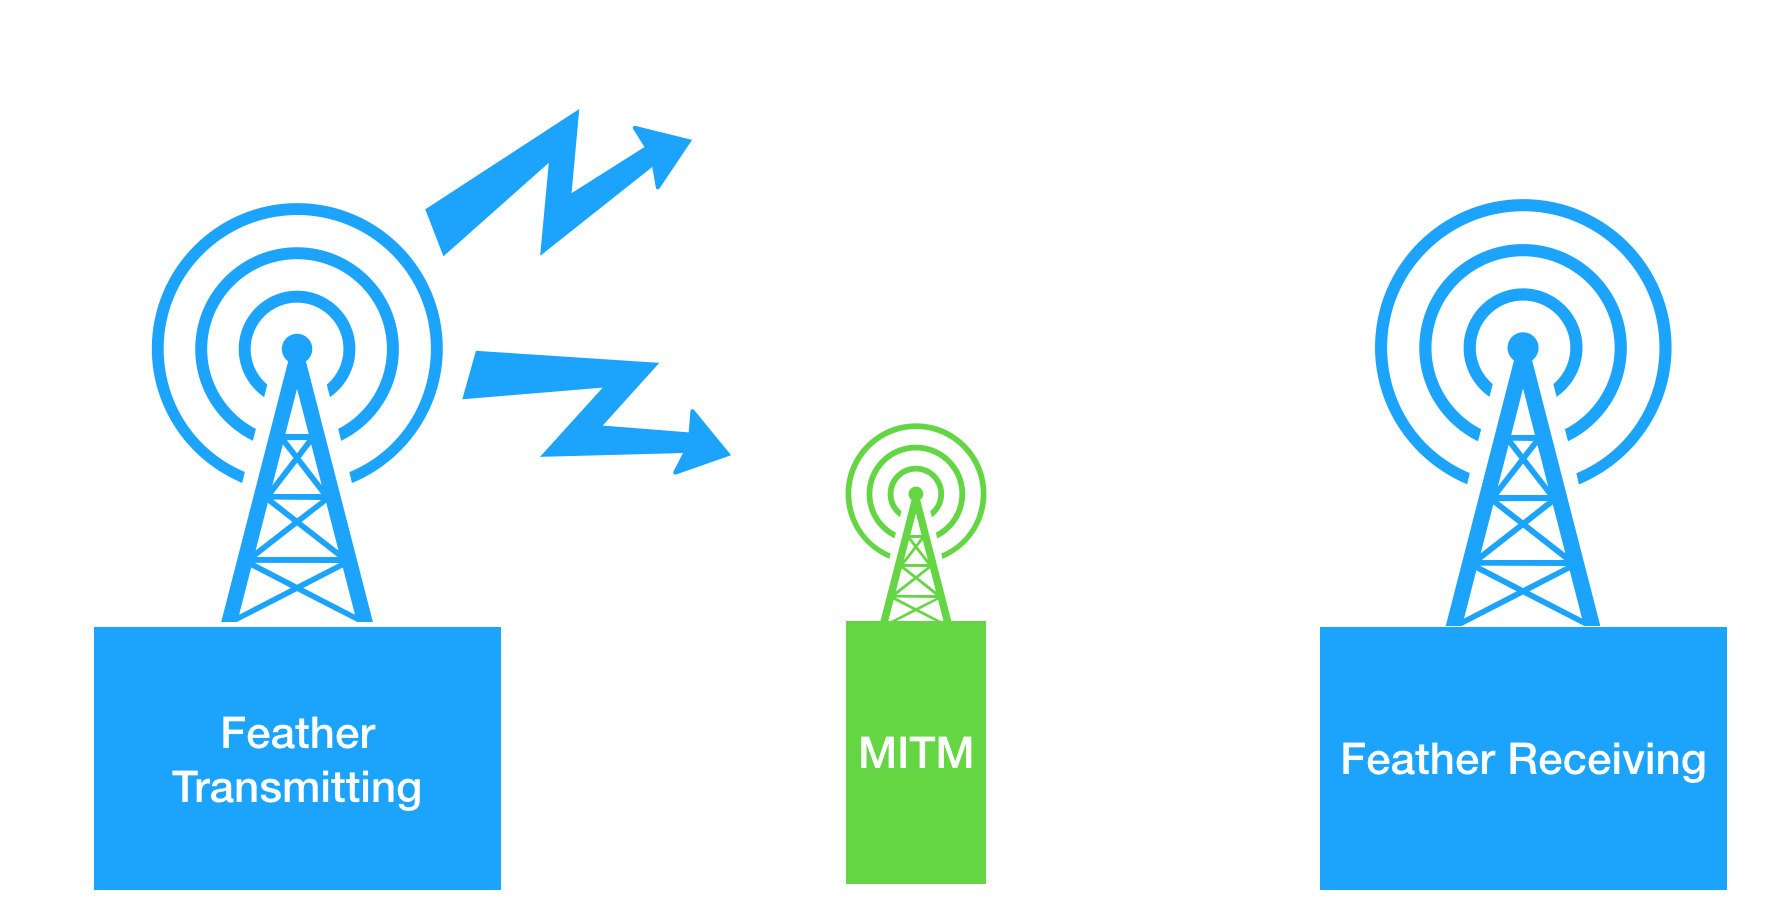
\includegraphics[width=\textwidth]{mitm.png}
\caption{MITM attack on our two feathers}
\label{mitm}
\centrefigureend

Using the gnuradio flow from before, find the frequency which the feather is transmitting on. It's probably going to be the loudest signal you can see, since the transmitter is close to the antenna. 

\subsection{Filtering}

The first step is to use an \gls{lpf} to make sure we receive only the transmission we are interested in. Drag an \gls{lpf} into the gnuradio flow, and add another QT Frequency Sink to see the output. In addition, it's a good idea to add some QT Range Widgets so you can change the parametres of the filter as it's running. Our aim for the \gls{lpf} is to have an output that looks abit like barad-dur.

\begin{figure}
    \centering
    \begin{minipage}{0.45\textwidth}
        \centering
        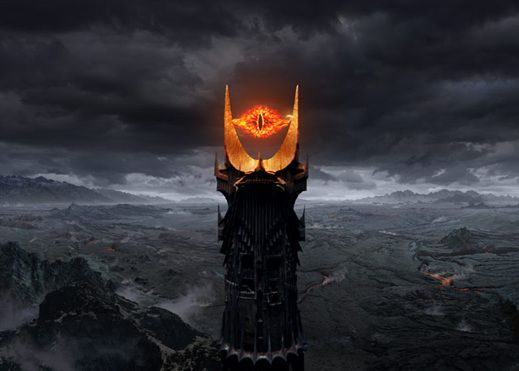
\includegraphics[width=\textwidth]{barad_dur.jpg} 
        \caption{Sauron's home.}
    \end{minipage}\hfill
    \begin{minipage}{0.45\textwidth}
        \centering
        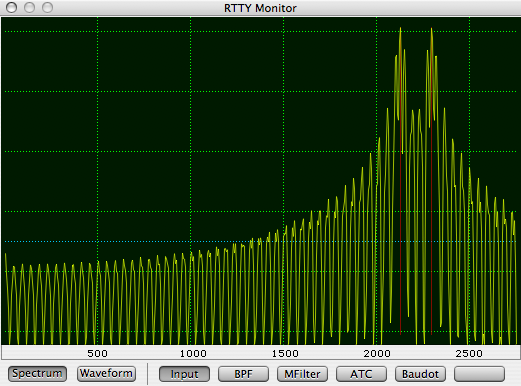
\includegraphics[width=\textwidth]{fsk_plot.png}
        \caption{FSK Signal as seen on a frequency plot.}
    \end{minipage}
\end{figure}